\documentclass[handout]{beamer}
%\usetheme{AnnArbor} % replace it with Boadilla if you want no section bar
%\usecolortheme{crane} % other ones: dove, dolphin, rose, seahorse, orchid, crane, seagull, lily, wolverine
%\usefonttheme{serif} 
\usetheme{CambridgeUS} % replace it with Boadilla if you want no section bar
\usefonttheme[onlymath]{serif} % uncomment if you want it just for math

\setbeamertemplate{navigation symbols}{}  % comment to have nagivation

\usepackage[compress,comma,authoryear]{natbib}
\usepackage{tikz}
\usetikzlibrary{fit,positioning}
\usepackage{amsmath,mathtools}
\usepackage{amsthm}
\usepackage{booktabs}
\usepackage{graphicx,epstopdf}
\usepackage{hyperref}


\definecolor{blue}{RGB}{0,114,178}
\definecolor{orange}{RGB}{213,94,0}
\definecolor{red}{RGB}{190,0,0}
\definecolor{yellow}{RGB}{240,228,66}
\definecolor{green}{RGB}{0,158,115}
\definecolor{Lblue}{RGB}{0,197,155}
\definecolor{Dblue}{RGB}{0,76,119}
\definecolor{Lgreen}{RGB}{180,255,230}

\hypersetup{
	colorlinks=false,
	linkbordercolor = {white},
	linkcolor = {blue}
}
\definecolor{MyBackground}{RGB}{245,245,245}

\setbeamercolor{frametitle}{fg=blue}
\setbeamercolor{title}{fg=blue}
\setbeamertemplate{footline}[frame number]
\setbeamertemplate{navigation symbols}{} 
\setbeamertemplate{itemize item}[circle]%{$\bigstar$}
\setbeamertemplate{itemize subitem}{$\bigstar$}
\setbeamercolor{itemize item}{fg=blue}
\setbeamercolor{itemize subitem}{fg=blue}
\setbeamercolor{enumerate item}{fg=blue}
\setbeamercolor{enumerate subitem}{fg=blue}
\setbeamercolor{button}{bg=MyBackground,fg=blue}
\setbeamercolor*{palette primary}{use=structure,fg=blue,bg=white}
\setbeamercolor*{palette secondary}{use=structure,fg=white,bg=Dblue}
\setbeamercolor*{palette tertiary}{use=structure,fg=white,bg=blue}
\setbeamercolor*{palette quaternary}{fg=white,bg=black}
\setbeamercolor*{palettes quaternary}{fg=white,bg=Lgreen}
%\setbeamercolor{titlelike}{parent=structure,bg=Lgreen}
%\setbeamercolor{title in head/foot}{bg=Lgreen,fg=orange}

\setbeamertemplate{enumerate item}{%
	\usebeamercolor[bg]{item projected}%
	\raisebox{1.5pt}{\colorbox{blue}{\color{fg}\footnotesize\insertenumlabel}}%
}



\begin{document}
	\title[Econometrics 2]{Econometrics 2 (M.Sc.)}
	\subtitle{Regression Discountinuity}
	\author[Mohammad Hoseini]{Mohammad Hoseini}
	
	%\institute[IMPS]{Institute for Management and Planning Studies (IMPS)}
	
\date[Spring 2024]{Spring 2024 \\
	\vspace{10pt} @metrics2
}

	
\begin{frame}[plain]
	\titlepage
\end{frame}

\section{Regression Discountinuity}
\subsection{Introduction}

\begin{frame}{Outline}

\begin{enumerate}
	\item Introduction
	\item Sharp RD
	\item Fuzzy RD
\end{enumerate}\bigskip


\end{frame}

\begin{frame}{Motivation}
So far we learned matching, IV,  and DiD to eliminate selection-on-unobservables bias.\bigskip

The choice of method is based on the context of the problem like whether there is a good IV or not, etc.\bigskip

Another method to eliminate selection bias that we cover in this lecture is called Regression Discountinuity design (RD or RDD).\bigskip

In RD the treatment is determined by a continuous variable crossing a cutoff, around which the just treated and just untreated are homogeneous.\bigskip

In other words, RD provides a local randomization at the expense of identifying the treatment only at the cutoff.
\end{frame}

\begin{frame}{Before-After estimator as a simple RD}
	Comparing $Y$ before and after the treatment.\medskip
	
	For example, suppose a speed limit law is assigned to decrease the speed limit in roads from 120 to 110 kmph.\medskip
	
	$Y$ is the number of car accidents. A simple estimator for the effect of the law is $\frac{1}{N}\sum_i Y_{ic}-Y_{ic-1}$\medskip
	
	The critical assumption for this estimator is that no other sudden change happens in the economy like a sudden change in weather or a holiday that raises/reduces the number of car trips.\medskip
	
	The identification assumption in before-after estimator:
	\[E(\Delta Y_t)=E(Y_c-Y_{c-1})=E(Y^1_c-Y^0_{c-1}) = E(Y^1_c-Y^0_c)-E(Y^0_c-Y^0_{c-1})\]
	$\Rightarrow$ The ID assumption is $E(Y^0_c)=E(Y^0_{c-1})$
	
\end{frame}



\begin{frame}{Event study}
A common use of before-after estimator is ``event study'' which concerns the impact of an event on the value of a firm.\bigskip
 
For instance, suppose there is an unexpected announcement of increased earning from a big company at $t_1$. One can gauge the effect of the earning announcement on the stock price $Y$ as  $Y_{t2}-Y_{t0}$.\medskip

But there should be no other change in the economy.
\begin{figure}
	\centering
	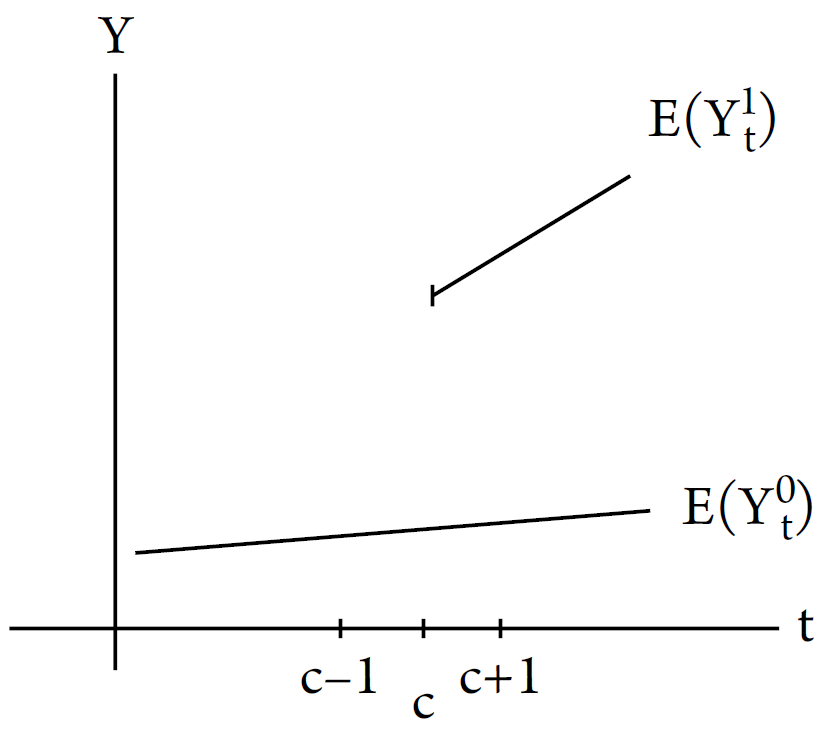
\includegraphics[width=0.4\linewidth]{./Figures/BAestimator}
	\caption{}
	\label{fig:baestimator}
\end{figure}

\end{frame}

\begin{frame}{Types of RD}
	RD is similar to before-after with time $t$ is replaced by a running/assignment variable $X$.\bigskip
	
	Types of RD:\begin{itemize}
		\item Sharp RD: treatment is a deterministic function of a covariate $X$.
		\item Fuzzy RD: exploits discontinuities in the probability of treatment conditional on a covariate $X$ (the discontinuity is then used as an IV).
	\end{itemize}\bigskip
	
	RD captures the causal effect by distinguishing the nonlinear and
	discontinuous function, $1(X_i \ge X_0)$ from the smooth function $f (X_i)$.
\end{frame}

\begin{frame}{Sharp RD}
	In Sharp RD designs you exploit that treatment status is a deterministic and discontinuous function of a covariate $X$.
	\[D_i=\begin{cases*}
	1 \text{ if } X_i\ge X_0\\
	0 \text{ if } X_i< X_0\\
		\end{cases*}\]
	$X_0$ is a known threshold or cutoff. Once we know $X_i$ we know $D_i$.\bigskip
	
%	As highlighted by Imbens and Lemieux (2008) 
	There is no value of $X_i$
	at which you observe both treatment and control observations. Thus, the method relies on extrapolation across covariate values.\medskip
	
%	For this reason we cannot be agnostic about regression functional form in RD.
\end{frame}

\begin{frame}{Sharp RD}
	Suppose that in addition to the assignment mechanism above,
	potential outcomes can be described by a linear, constant effects
	model:
	\[E[Y^0_i|X_i ] = \alpha + \beta X_i, \quad
	Y^1_i = Y^0_i + \rho\]
	This leads to the regression:
	\[Y_i = \alpha + \beta X_i + \rho D_i + \eta_i\]
	The key difference between this regression and regressions we have
	investigated in previous lectures is that $D_i$ is not only correlated with $X_i$ but it is a deterministic function of $X_i$.\bigskip
	
	In general $E[Y^0_i|X_i ] = f (X_i)$ can be nonlinear for some 	reasonably smooth function $f (X_i )$ and we can construct RD estimates by fitting:
	\[Y_i = f(X_i) + \rho D_i + \eta_i\]
\end{frame}

\begin{frame}{Sharp RD example}
	\begin{columns}
		\begin{column}{.4\textwidth}
In non-linear case, there are 2 ways of approximating $f(X_i)$:

\begin{itemize}
	\item nonparametric kernel method
	\item pth order polynomial:\end{itemize}
	\[f(x_i)=\beta_0+\beta_1x_i+\dots+\beta_nx_i^n\]


		\end{column}
		\begin{column}{.6\textwidth}
		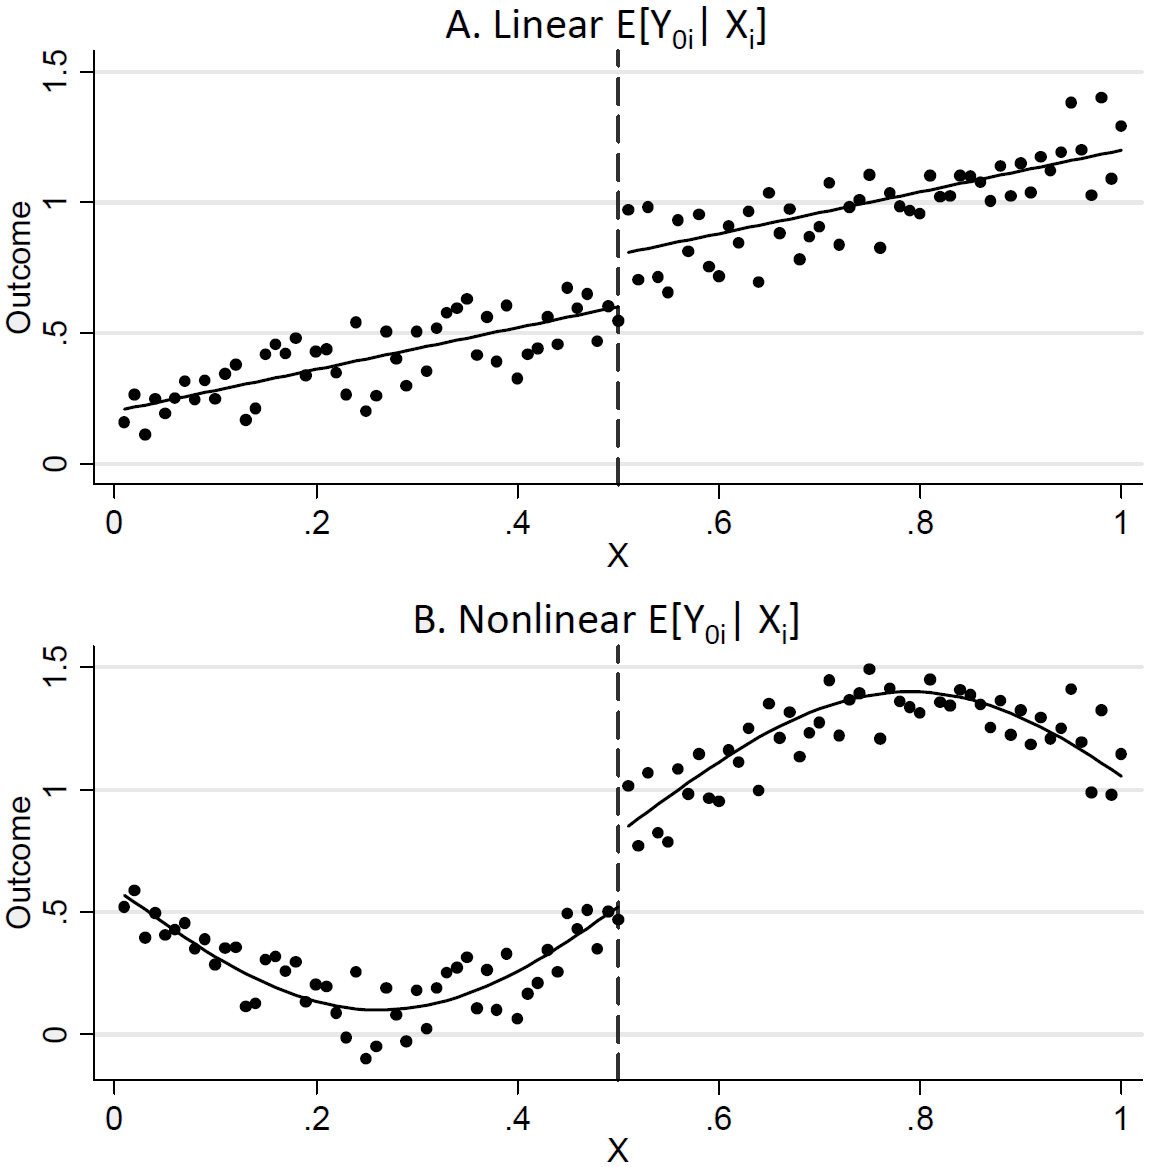
\includegraphics[width=\linewidth]{./Figures/RDsharp}
		\end{column}
	\end{columns}
\end{frame}

\begin{frame}{RD identification assumption}
	Key identifying assumption:
	$E[Y^0_i|X_i ]$ and $E[Y^1_i|X_i ]$ are continuos in $X_i$ at $X_0$.\medskip
	
	This means that all other unobserved determinants of $Y$ are
	continuously related to the running variable $X$.\medskip
	
	This allows us to use average outcomes of units just below the cutoff
	as a valid counterfactual for units right above the cutoff.\medskip
	
	This assumption cannot be directly tested. But there are some tests
	which give suggestive evidence whether the assumption is satisfied.
\end{frame}

\begin{frame}{Internal Validity of RD}
	The validity of RD estimates depends crucially on the assumption 	that the polynomials provide an adequate representation of $E[Y^0_i|X_i ]$.\medskip 
	
	If not what looks like a jump may simply be a non-linearity in $f(X_i)$
	that the polynomials have not accounted for.\medskip
	
	To reduce the likelihood of such mistakes, we can look at data in a small neighborhood around discontinuity.\medskip
	
\begin{center}
		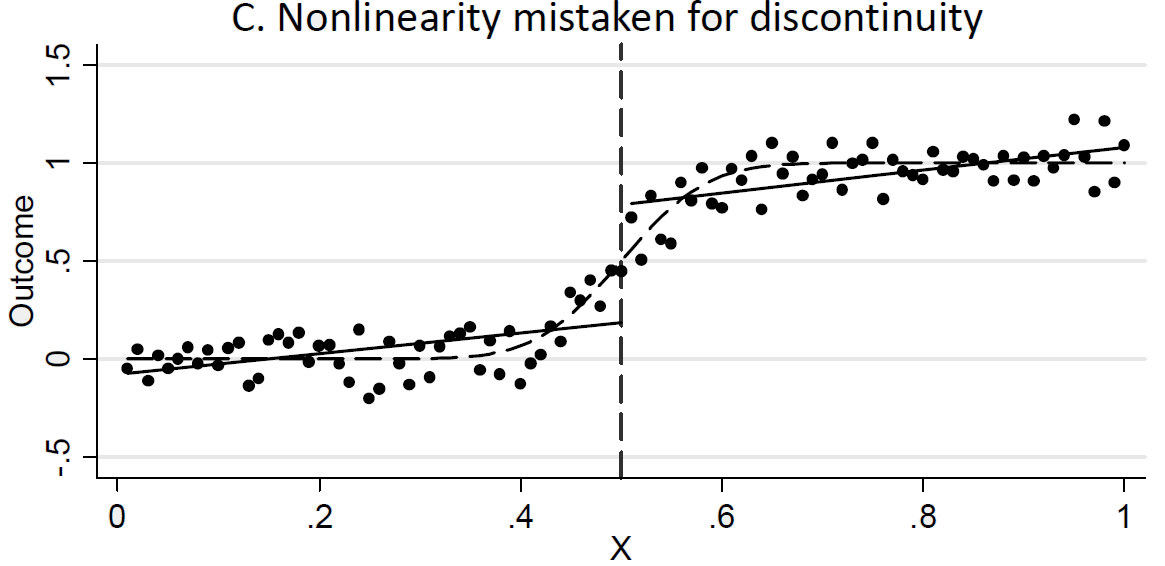
\includegraphics[width=.7\linewidth]{./Figures/RDsharp1}
\end{center}

\end{frame}

\begin{frame}{Lee (2008)}
	Lee (2008) uses a sharp RD design to estimate the probability that the incumbent party wins an election.\medskip
	
	Incumbents may use privileges and resources of office to gain an advantage over other parties.\medskip
	
	Selection bias in OLS: Incumbents have already won an election and so they can better satisfy voters.\medskip
	
	Using data of US congressional elections, Lee (2008) looks at the likelihood a Democratic candidate wins as a function of relative vote share in the previous election.\medskip
	
	Discontinuity: Winner is determined by the difference between Democratic and Republican vote shares. 
	
	$D_i=1[$Democrat share $>$ Republican share$]$
\end{frame}

\begin{frame}{Lee (2008)}
	\begin{figure}
		\centering
		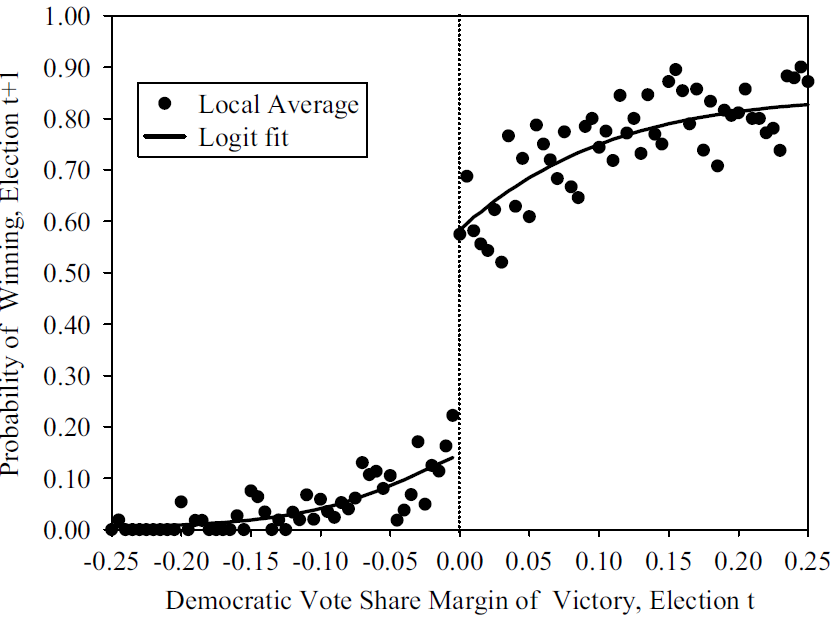
\includegraphics[width=0.7\linewidth]{./Figures/Lee2008}
	\end{figure}
The dots are average win rate within each share margin bin (width 0.005).

The fitted values are from a 4th order polynomial and cutoff indicator $D_i$.	
\end{frame}

\begin{frame}{Lee (2008)}
	The probability of a democratic win is increasing in past vote share. \medskip
	
	There is a dramatic jump in win rates at the 0 percent mark, the point where a Democratic candidate gets more votes.\medskip 
	
	Based on the size of the jump, incumbency appears to raise party re-election probabilities by about 40 percentage points.
	\begin{columns}
		\begin{column}{.45\textwidth}
	A identification check: Democratic wining in older elections should be unrelated to the margin-of-victory cutoff in the last election.
%	the average number of terms the candidate has served in Congress, it can be between 0 and 1 because they are averages over bins.
		\end{column}
		\begin{column}{.55\textwidth}
		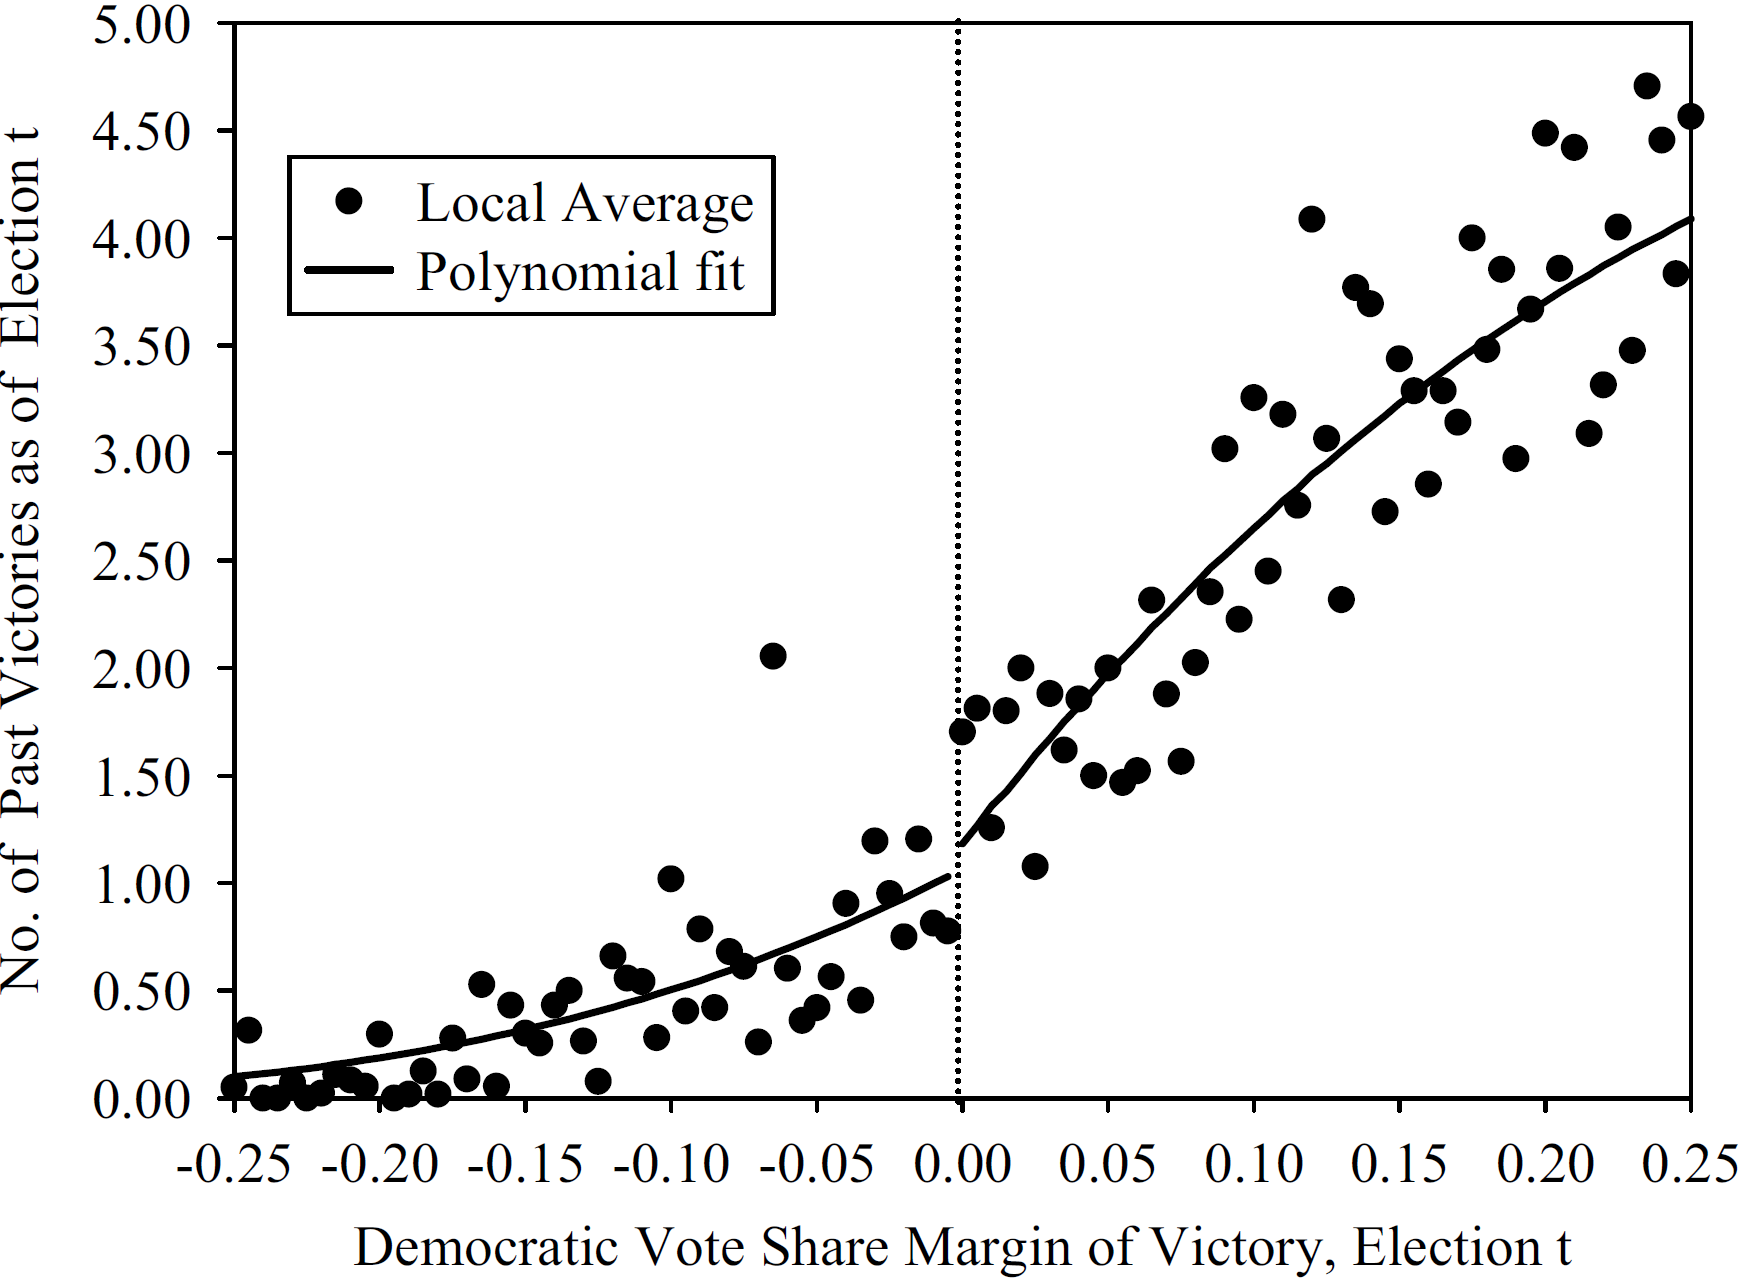
\includegraphics[width=\linewidth]{./Figures/Lee2008_}
		\end{column}
	\end{columns}	
\end{frame}

\begin{frame}{Fuzzy RD}
	Fuzzy RD exploits discontinuities in the probability of treatment conditional on a covariate.\medskip
	
	The discontinuity becomes an instrumental variable for treatment status.\medskip
	
	$D_i$ is no longer deterministically related to crossing a threshold but there is a jump in the probability of treatment at $X_0$.
		\[D_i=\begin{cases*}
	g_1(x_i) \text{ if } x_i\ge x_0\\
	g_0(x_i) \text{ if } x_i< x_0\\
	\end{cases*}, \quad g_0(x_i)\ne g_1(x_i) \]
The more $g_0$ and $g_1$ are different at $x_0$, the better.\medskip
	
\end{frame}


\begin{frame}{Use the Discontinuity as Instrument}
	We can write down a first stage relationship:
	\[E[D_i|x_i ] = \gamma_{0}+\gamma_1 x_i+\gamma_2 x_i^2+\dots+\gamma_px_i^p+\pi T_i+\varepsilon_{1i} \] One can therefore use $T_i=1[x_i>x_0]$ as instruments for $D_i$.\medskip
	%One can therefore use both $T_i=1[x_i>x_0]$ as well as the interaction terms as instruments for $D_i$.\medskip
	
	The second stage relationship:
	\[ Y_i=\beta_0+\beta_1 x_i+\beta_2 x_i^2+\dots+\beta_p x_i^p+\rho D_i+\varepsilon_{2i} \]
	
	The fuzzy RD reduced-form is then:
	\[Y_i = \mu + \kappa_1x_i + \kappa_2x_i^2+\dots+\kappa_p x_i^p+\rho\pi T_i+\varepsilon_{3i} \]
	where $\mu =\beta_0 + \rho \gamma_{0}$ and $\kappa_j =\beta_j + \rho \gamma_{j}$ for $j=1,\dots,p$.
	
\end{frame}

\begin{frame}{Angrist and Lavy (1999)}
A fuzzy RD design to analyze the effect of class size on test scores.\medskip

An old Talmudic rule says classes should be split if they have more than 40 students. Thus, in Israel:
\begin{itemize}
	\item A school with 40 students has only one class.
	\item A school with 41 students has two classes of sizes 21 and 20.
\end{itemize}\bigskip

Predicted class size from the rule with enrollment $e_s$ is:
\[m_{sc} = \frac{e_s}{\text{int}[\frac{e_s-1}{40}]+1}\]



\end{frame}

\begin{frame}{Angrist and Lavy (1999)}
Because the rule is not followed strictly they use a fuzzy discontinuity design.
\begin{figure}
	\centering
	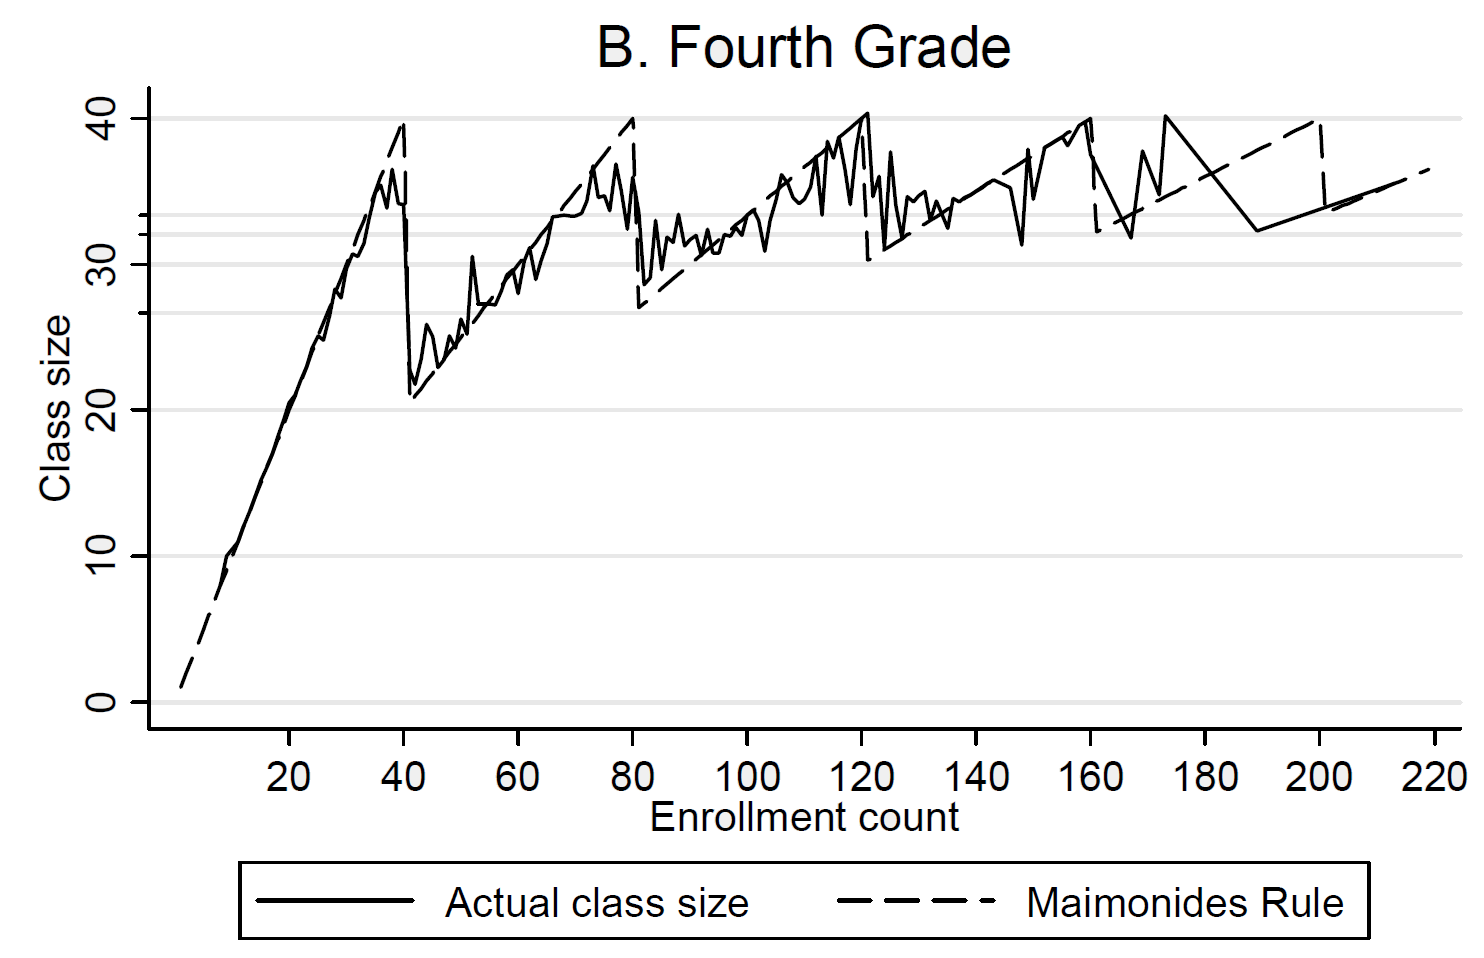
\includegraphics[width=0.8\linewidth]{./Figures/angristlavy}
\end{figure}

\end{frame}	

\begin{frame}{Econometric specification}
They want to estimate the relationship between average achievement and class size.\bigskip
\[Y_{isc}= \alpha_0 + \rho n_{sc} + \eta_{isc} \]

Estimating this relationship with OLS may lead to biased results because class size is likely to be correlated with the error term:
\begin{itemize}
	\item Parents from higher socioeconomic backgrounds may put their children in schools with smaller classes.
	\item  Because principals may put weaker students in smaller classes.
\end{itemize}

The causal variable of interest (class size) takes on many values. Thus, in the First stage, they exploit discontinuities in average class size instead of probabilities of a single treatment and they use multiple discontinuities.
\end{frame}

\begin{frame}{Fuzzy RD design}
Angrist and Lavy therefore use the rule in a fuzzy RD design.
\[ Y_{isc} = \alpha_0 + \alpha_1d_s + \rho n_{sc} + \beta_1e_s + \beta_2e^2_s + \eta_{isc} \]
where $Y_{isc}$ is the test score of student $i$ in school $s$ and class $c$. $n_{sc}$ is class size. $e_s$ is enrollment in school $s$. $d_s$ is the percentage of disadvantage students in class.\medskip

The variables relate to the previous description as follows:
\begin{itemize}
	\item $n_{sc}$ plays the role of $D_i$.
	\item $e_s$ plays the role of $X_i$.
	\item $m_{sc}$ plays the role of $T_i$.
\end{itemize}
The first stage regression is:
\[n_{sc} = \gamma_0 + \gamma_1 d_s + \pi m_{sc} + \delta_1e_s + \delta_2e^2_s + \zeta_{isc}\]
where $m_{sc}$ is the function describing the rule.
\end{frame}

\begin{frame}{Angrist and Lavy (1999)}
\begin{figure}
	\centering
	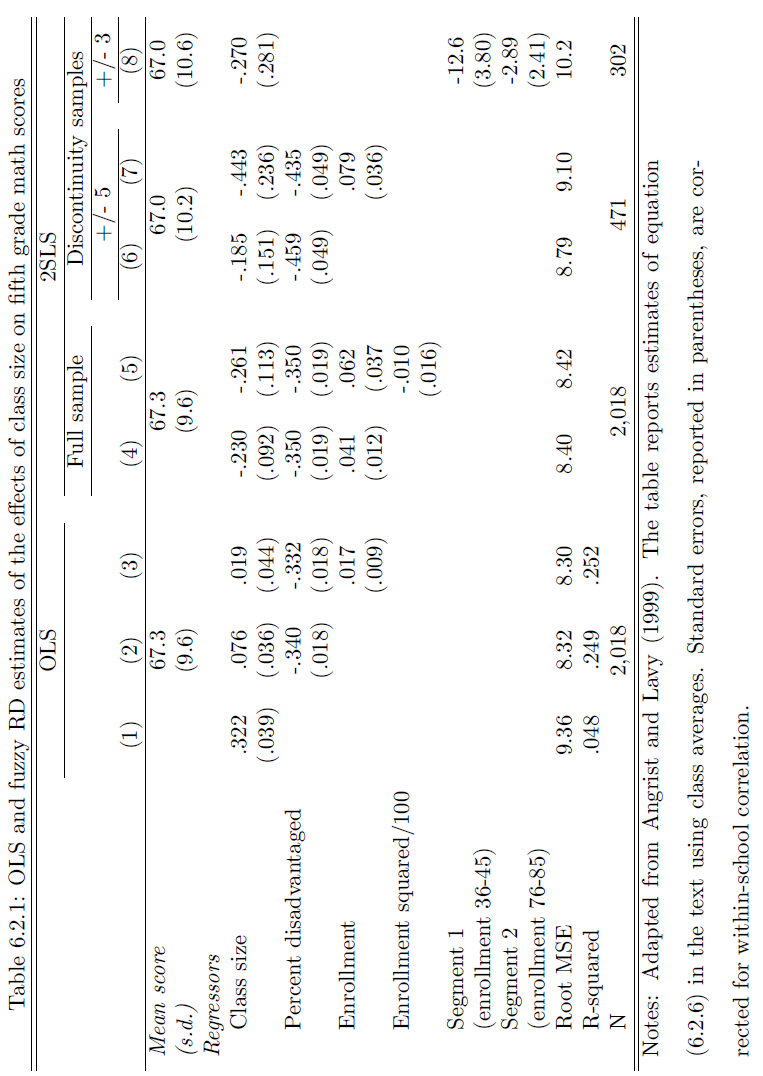
\includegraphics[angle=270,width=.85\linewidth]{./Figures/angristlavy1}
\end{figure}

\end{frame}

\begin{frame}{Practical tips}
	It is probably advisable to report results for both estimation types:
	\begin{itemize}
		\item Polynomials in X.
		\item Local linear regression.
	\end{itemize}
	In robustness checks you also want to show that including higher
	order polynomials does not substantially affect your findings.\bigskip
	
	You also want to show that your results are not affected if you vary the window around the cutoff (standard errors may go up but
	hopefully the point estimate does not change).
\end{frame}

\begin{frame}{Regression Kink Design}
A variant of the RD design is regression kink design (RKD).\bigskip

Instead of a jump in the outcome you now expect a jump in the first derivative.\bigskip

Using a kink in some policy rule to identify the causal effect of the policy.
\begin{itemize}
	\item Card, Lee, Pei and Weber (2015) study the impact of unemployment benefits on the length of unemployment in Austria with this approach
\end{itemize}


\end{frame}


\begin{frame}{Causal inference flowchart}
	\scriptsize
	\begin{tikzpicture}[
		node distance = 5mm and -3mm,
		every path/.style = {draw, -latex} ]
		\node (begin) [draw=black, rounded corners] {\textit{begin}};
		
		\pause;
		
		\node (start) [draw=black, rounded corners, text width=4cm, below =2mm of begin] {\textit{Can you randomize treatment (T) and control (C) groups?} };
		\draw   (begin) -- (start);		
		
		\pause;
		
		\node (RCT) [left=12mm of start, draw=black, text width=2cm, align=center, fill=gray!30]  {\textbf{Randomized experiment}}; 
		\draw   (start) -- (RCT) node [above, midway] {Yes};
		
		\pause;
		
		\node (natural) [draw=black, rounded corners, text width=4cm, below right=of start] {\textit{Is the an exogeneous shock (natural experiment) that randomly separate T and C?} };
		\draw   (start) -| (natural) node [above, midway] {No};
		
		\pause;
		
		\node (cutoff) [draw=black, rounded corners, text width=2.5cm, left =2cm of natural] {\textit{Is there a cuttoff that seperates T and C?} };
		
		\draw   (natural) -- (cutoff) node [above, midway] {Yes};
		
		\pause	;	
		
		\node (DID) [left=7mm of cutoff, draw=black, text width=2cm, align=center, fill=gray!30]     {\textbf{Difference-in-difference}};
		\draw   (cutoff) -- (DID) node [above, midway] {No};		
		
		\pause	
		\node (null) [below =of natural] {};		
		\node (RD) [left=5.7cm of null, draw=black,  rounded corners, text width=3cm, align=center]  {\textit{Is there full complinace around the cutoff?}}; 		
		\draw   (cutoff) |- (RD) node [above right, midway] {Yes};
		
		\pause		;
		
		\node (SRD) [below =2.5cm of DID, draw=black, text width=2cm, align=center, fill=gray!30]  {\textbf{Regression Discountinuity (sharp)}}; 			
		\draw   (RD) -- (SRD) node [left, midway] {Yes};				
		
		\pause		;
		
		\node (FRD) [right=5mm of SRD, draw=black, text width=2cm, align=center, fill=gray!30]  {\textbf{Regression Discountinuity (fuzzy)}}; 		
		\draw   (RD) -- (FRD) node [right, midway] {No};		
		
		\pause		;
		
		\node (ivar) [draw=black, rounded corners, text width=4cm, below =of natural] {\textit{Is there some variable to predict treatment not directly corrolated with the outcome?} };	
		\draw   (natural) -- (ivar) node [left, midway] {No};
		
		\pause		;
		
		\node (IV) [left=7mm of ivar, draw=black, text width=1.6cm, align=center, fill=gray!30]     {\textbf{Instrumental variable}};		
		\draw   (ivar) -- (IV) node [above, midway] {Yes};
		\draw[dashed]   (FRD) -- (IV);
		\pause		;
		
		\node (match) [draw=black, rounded corners, text width=4cm, below =of ivar] {\textit{Do we have information to find similar individuals in T and C?} };	
		\draw   (ivar) -- (match) node [left, midway] {No};
		\pause		;
		
		\node (PSM) [left=7mm of match, draw=black, text width=1.2cm, align=center, fill=gray!30]  {\textbf{Matching}}; 		
		\draw   (match) -- (PSM) node [above, midway] {Yes};
		\pause		;		
		
		\node (end) [below=3mm of match, text width=4cm, draw=black, fill=gray!30]  {\vspace{-3pt}
			\begin{columns}
				\begin{column}{0.05\textwidth}\end{column}
				\begin{column}{0.95\textwidth}
					\textbf{Use regression and convince us that CIA holds}
				\end{column}
%				\begin{column}{0.4\textwidth}
%					
\includegraphics[width=.85\linewidth]{../figure/frown}
%				\end{column}
			\end{columns}\vspace{-5pt}};
		%
		
		%%
		
		
		
		
		
		\draw   (match) -- (end) node [left, midway] {No};
		
		
		
		
		
		
		
	\end{tikzpicture}
	
\end{frame}

\end{document}
